\documentclass{article}
\usepackage{setspace}
\usepackage{amsmath}
\usepackage{amssymb}
\usepackage{amsthm}
\usepackage{graphicx} 
\usepackage{float} 
\usepackage{fancyhdr}                                
\usepackage{lastpage}        
\usepackage{textcomp}                               
\usepackage{layout}   
\usepackage{subfigure} 
\pagestyle{fancy}  
\lhead{ZHANG HUAKANG}
\chead{Assignment 2} 
\rhead{DB92760} 
\renewcommand{\baselinestretch}{1.05}
\title{Assignment 2 of CISC 1006}
\author{ZHANG HUAKANG \\ DB92760 \\ \\ Computer Science, \\Faculty of Science and Technology}
\begin{document}
    \maketitle
    \section{}
    Let $A$ be the event thatan automobile being filled with gasoline will also need an oil change, and $B$ be the event that  it needs a new oil filter.
    \begin{equation*}
        \begin{split}
            P(A)=&0.25\\
            P(\overline{A})=&0.75\\
            P(B)=&0.4\\
            P(\overline{B})=&0.6\\
            P(A\cap B)=&0.14
        \end{split}
    \end{equation*}
        \subsection{}
            \paragraph{
                \begin{equation*}
                    \begin{split}
                        P(B|A)=&\frac{P(A\cap B)}{P(A)}\\
                            =&\frac{0.14}{0.25}\\
                            =&0.56\\
                    \end{split}
                \end{equation*}
            }
        \subsection{}
            \paragraph{
                \begin{equation*}
                    \begin{split}
                        P(A|B)=&\frac{P(A\cap B)}{P(B)}\\
                            =&\frac{0.14}{0.4}\\
                            =&0.35\\
                    \end{split}
                \end{equation*}
            }
    \section{}
        Let $A_n$ be  the event that the probability that a specific engine is available when needed, where $n=1,2$
        \begin{equation*}
            \begin{split}
                P(A_n)=&0.96\\
                P(\overline{A_n})=&0.04\\
            \end{split}
        \end{equation*}
        \subsection{}
            \paragraph{
                \begin{equation*}
                    \begin{split}
                        P_a=&P(\overline{A_1}\cap \overline{A_2})\\
                    \end{split}
                \end{equation*}
                Because fire enginer operates independently.
                \begin{equation*}
                    \begin{split}
                        P(\overline{A_1}\cap \overline{A_2})=&P(\overline{A_1})\times P(\overline{A_2})\\
                        =&0.04^2\\
                        =&1.6\times 10^{-3}
                    \end{split}
                \end{equation*}
            }
        \subsection{}
            \paragraph{
                \begin{equation*}
                    \begin{split}
                        P_b=&1-P_a\\
                        =&0.9984\\
                    \end{split}
                \end{equation*}
            }
    \section{}
        \paragraph{
            \begin{figure}[H]
                \centering
                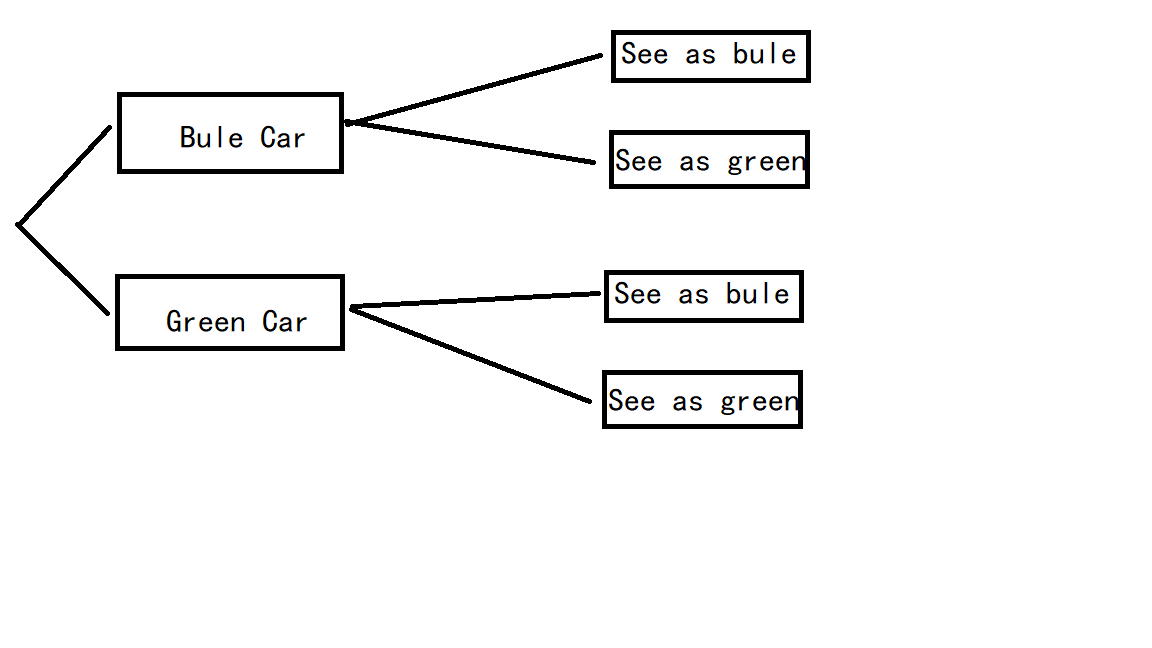
\includegraphics[width=0.9\textwidth]{img/Assignment2-01.png}
            \end{figure}
            Let $A$ be the event that the witness sees a car as blue, and $B$ be the event that the car is blue.
            we can know that 
            \begin{equation*}
                \begin{split}
                    P(B)=&\frac{1}{1+99}\\
                        =&0.01\\
                    P(\overline{B})=&0.99\\
                    P(A|B)=&0.99\\
                    P(A|\overline{B})=&0.02\\
                    P(\overline{A}|B)=&0.01\\
                    P(\overline{A}|\overline{B})=&0.98\\
                \end{split}
            \end{equation*}
            \begin{equation*}
                \begin{split}
                    P(B|A)=&\frac{P(B\cap A)}{P(A)}\\
                        =&\frac{P(B)P(A|B)}{P(A)}\\
                        =&\frac{P(B)P(A|B)}{P(A\cap B)+P(A\cap \overline{B})}\\
                        =&\frac{P(B)P(A|B)}{P(B)P(A|B)+P(\overline{B})P(A|\overline{B})}\\
                        =&\frac{1}{3}
                \end{split}
            \end{equation*}
            Thus the probability that when a car is blue the witness see it as bule is only $\frac{1}{3}$ which is a very low probability. So the probability that the car driver is innocence is $\frac{2}{3}$
        }
    \section{}
        \paragraph{
            \begin{figure}[H]
                \centering
                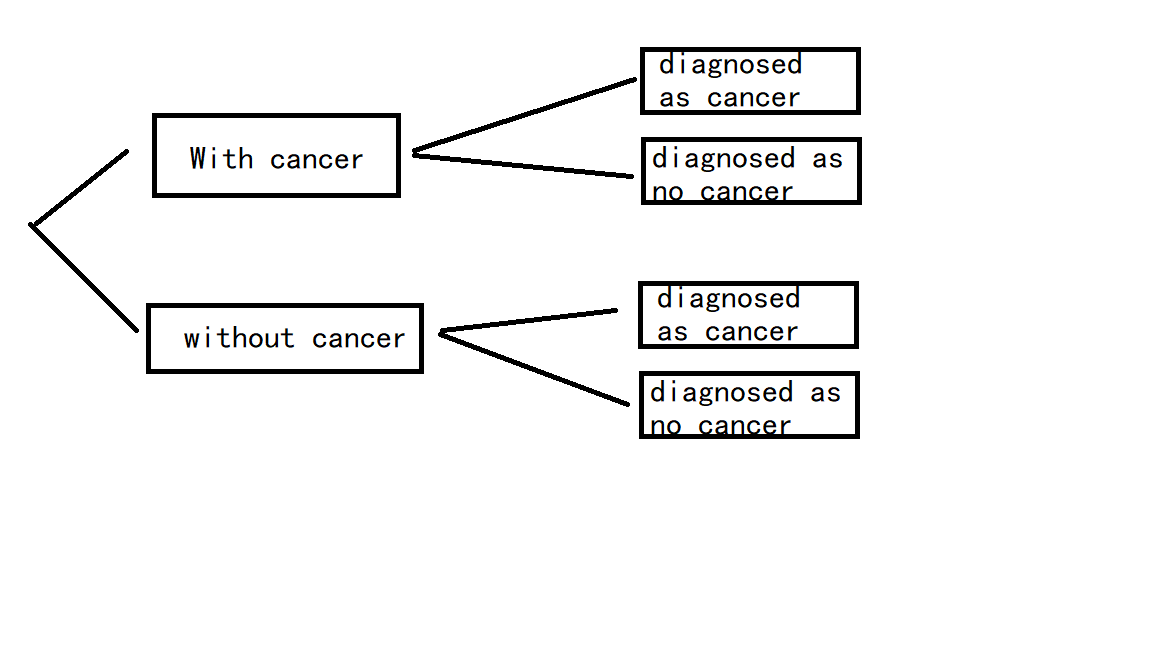
\includegraphics[width=0.9\textwidth]{img/Assignment2-02.png}
            \end{figure}
            Let $C$ be the event that a person has cancer, $D$ is that a person is diagnosed as cancer.
            \begin{equation*}
                \begin{split}
                    P(C)=&0.05\\
                    P(\overline{C})=&0.95\\
                    P(D|C)=&0.78\\
                    P(\overline{D}|C)=&0.22\\
                    P(D|\overline{C})=&0.06\\
                    P(\overline{D}|\overline{C})=&0.94\\
                    P(D)=&P(D\cap C)+P(D\cap \overline{C})\\
                        =&P(C)P(D|C)+P(\overline{C})P(D|\overline{C})\\
                        =&0.096\\
                    P(C|D)=&\frac{P(C\cap D)}{P(D)}\\
                        =&\frac{P(C)P(D|C)}{P(D)}\\
                        =&0.40625\\
                \end{split}
            \end{equation*}
        }
    \section{}
        \subsection*{}
            \paragraph{
                \begin{figure}[H]
                    \centering
                    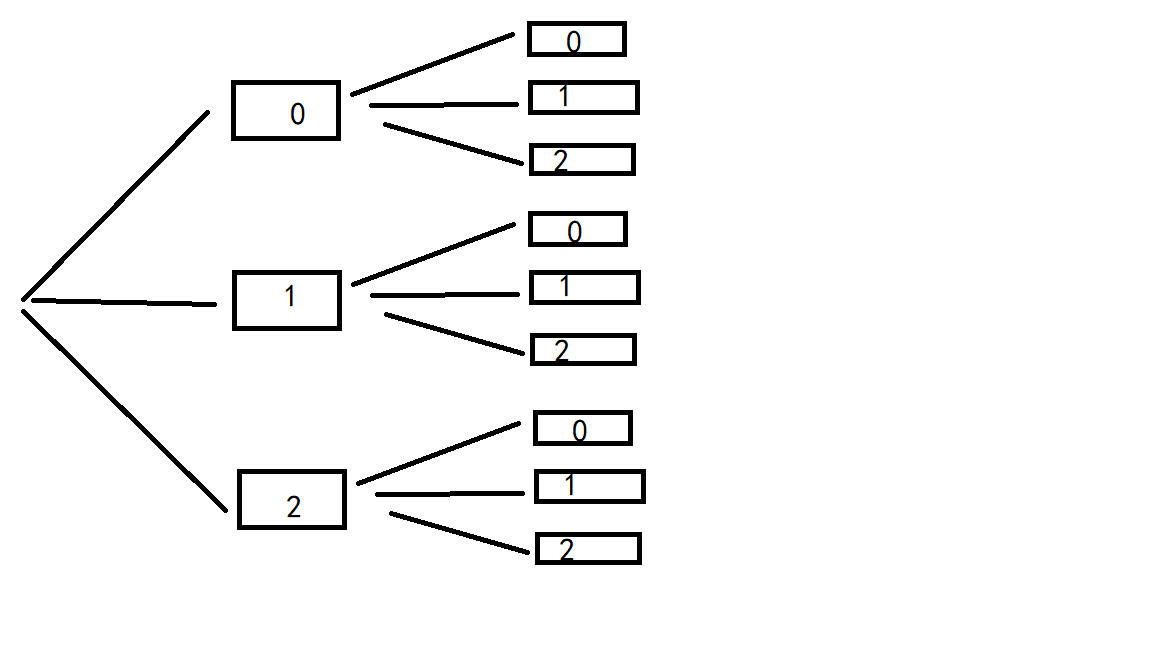
\includegraphics[width=0.9\textwidth]{img/Assignment2-03.png}
                \end{figure}
                Let $D_n$ be the event that lots contain $n$ defective components and $d_n$ be the event that $n$ defective exist in the lot.
                \begin{equation*}
                    \begin{split}
                        P(D_0)=&0.6\\
                        P(D_1)=&0.3\\
                        P(D_2)=&0.1\\
                        P(d_0|D_0)=&1\\
                        % P(d_1|D_0)=&0\\
                        % P(d_2|D_0)=&0\\
                        P(d_0|D_1)=&\frac{C_{19}^2C_1^0}{C_{20}^2}\\
                            =&0.9\\
                        P(d_0|D_2)=&\frac{C_{18}^2C_2^0}{C_{20}^2}\\
                            =&\frac{153}{190}\\
                        P(d_0)=&P(D_2)P(d_0|D_2)+P(D_1)P(d_0|D_1)+P(D_0)P(d_0|D_0)\\
                            =&\frac{903}{950}\\
                    \end{split}
                \end{equation*}
            }
        \subsection{}
            \begin{equation*}
                \begin{split}
                    P(D_0|d_0)=&\frac{P(D_0\cap d_0)}{P(d_0)}\\
                        =&\frac{P(D_0)P(d_0|D_0)}{P(d_0)}\\
                        =&\frac{190}{301}\\
                \end{split}
            \end{equation*}
        \subsection{}
            \begin{equation*}
                \begin{split}
                    P(D_1|d_0)=&\frac{P(D_1\cap d_0)}{P(d_0)}\\
                        =&\frac{P(D_1)P(d_0|D_1)}{P(d_0)}\\
                        =&\frac{171}{602}\\
                \end{split}
            \end{equation*}
        \subsection{}
            \begin{equation*}
                \begin{split}
                    P(D_2|d_0)=&\frac{P(D_2\cap d_0)}{P(d_0)}\\
                        =&\frac{P(D_2)P(d_0|D_2)}{P(d_0)}\\
                        =&\frac{51}{602}\\
                \end{split}
            \end{equation*}
    \section{}
        \subsection{}
            \begin{equation*}
                \begin{split}
                    P(W)=&P(A\cap D\cap B\cap C)+P(A\cap D\cap \overline{B}\cap C)+P(A\cap D\cap B\cap \overline{C})\\
                        =&P(A)\times P(D)\times(P(B)P(C)+P(\overline{B})P(C)+P(B)P(\overline{C}))\\
                        =&\frac{2538}{3125}
                \end{split}
            \end{equation*}
        \subsection{}
            $$P(W|\overline{A})=0$$
        \subsection{}
            $$P(\overline{A}|W)=0$$
\end{document}